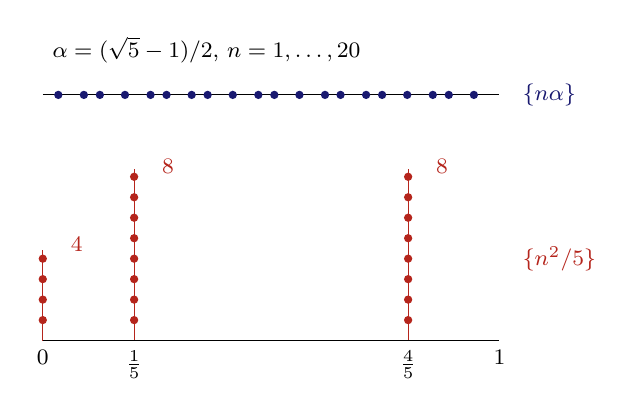
\begin{tikzpicture}[x=5.8cm,y=0.26cm,every node/.style={font=\footnotesize}]
  \draw (0,12)--(1,12);
  \foreach \x in {0.618,0.236,0.854,0.472,0.090,0.708,0.326,0.944,0.562,0.180,0.798,0.416,0.034,0.652,0.271,0.889,0.507,0.125,0.743,0.361} {
    \fill[MidnightBlue] (\x,12) circle (1.5pt);
  }
  \node[anchor=west,MidnightBlue] at (1.03,12) {$\{n\alpha\}$};
  \draw[BrickRed] (0,0)--(0,4.4);
  \draw[BrickRed] (0.2,0)--(0.2,8.4);
  \draw[BrickRed] (0.8,0)--(0.8,8.4);
  \foreach \k in {1,...,4} {\fill[BrickRed] (0,\k) circle (1.5pt);}
  \foreach \k in {1,...,8} {\fill[BrickRed] (0.2,\k) circle (1.5pt);}
  \foreach \k in {1,...,8} {\fill[BrickRed] (0.8,\k) circle (1.5pt);}
  \node[anchor=west,BrickRed] at (0.04,4.7) {$4$};
  \node[anchor=west,BrickRed] at (0.24,8.5) {$8$};
  \node[anchor=west,BrickRed] at (0.84,8.5) {$8$};
  \draw (0,0)--(1,0);
  \node[below] at (0,0) {$0$};
  \node[below] at (0.2,0) {$\frac15$};
  \node[below] at (0.8,0) {$\frac45$};
  \node[below] at (1,0) {$1$};
  \node[anchor=west,BrickRed] at (1.03,4) {$\{n^2/5\}$};
  \node[anchor=west] at (0,14.2) {$\alpha=(\sqrt5-1)/2$, $n=1,\ldots,20$};
\end{tikzpicture}
